\documentclass[14pt]{extarticle}
\usepackage{fontspec}
\usepackage{polyglossia}
\usepackage{amsmath}
\usepackage{amssymb}
\usepackage{xcolor}
\usepackage{fancyhdr}
\usepackage{graphicx}
\usepackage{listings}
\usepackage[most]{tcolorbox}
% \usepackage{setspace}
\usepackage{pifont}
\usepackage{enumitem}
\usepackage{titlesec}
\usepackage[bottom]{footmisc}
\usepackage{titling}
\usepackage{minted}
\usepackage{etoolbox}
\usepackage{array}
\usepackage{extsizes}
\usepackage{float}
\usepackage{booktabs}
\usepackage{hyperref}
\usepackage[onehalfspacing]{setspace}
\usepackage[a4paper, top=2.7cm, bottom=2.7cm, left=2.5cm, right=2.5cm, headheight=1.5cm, headsep=0.5cm]{geometry}
\usepackage{tikz}

\usetikzlibrary{automata, positioning, arrows.meta, arrows}

\newfontfamily\emoji{Segoe UI Emoji}

\pagestyle{fancy}

\setmainlanguage[numerals=western]{arabic}
\setotherlanguage{english}
% \newfontfamily\arabicfont[Script=Arabic]{Amiri}
\newfontfamily\arabicfont[Script=Arabic]{Calibri}
\newfontfamily\arabicfonttt[Script=Arabic]{Courier New}

\lstset{
  language=[Sharp]C,
  numbers=left,
  stepnumber=1,
  numbersep=8pt,
  frame=single,
  basicstyle=\ttfamily\small,
  keywordstyle=\color{blue},
  stringstyle=\color{red},
  commentstyle=\color{green!50!black}
}

\newif\ifdetailed
\ifdefined\setdetailed
  \setdetailed
\fi

\newif\ifwithsols
\ifdefined\setwithsols
  \setwithsols
\fi

% unified tcolorboxes for articles
\tcbset{colback=white, colframe=black, fonttitle=\bfseries, boxrule=0.8pt}
\newtcolorbox{boxDef}[1][]{colback=blue!5!white,colframe=blue!75!black,
  title={{\emoji📘} تعريف\ifx\\#1\\\else ~#1\fi :}}
\newtcolorbox{boxExercise}[1][]{colback=cyan!5!white,colframe=cyan!70!black,
  title={{\emoji🧩} تمرين\ifx\\#1\\\else ~#1\fi :}}
\newtcolorbox{boxExample}[1][]{colback=yellow!5!white,colframe=orange!90!black,
  title={{\emoji📝} مثال\ifx\\#1\\\else ~#1\fi :}}
\newtcolorbox{boxNote}[1][]{colback=gray!10!white,colframe=black,
  title={{\emoji✨} ملاحظة\ifx\\#1\\\else ~#1\fi :}}
\newtcolorbox{boxAttention}[1][]{colback=magenta!10!white,colframe=magenta!80!black,
  title={{\emoji🔔} تنبيه\ifx\\#1\\\else ~#1\fi :}}
\newtcolorbox{boxWarning}[1][]{colback=red!5!white,colframe=red!75!black,
  title={{\emoji⚡} ملاحظة هامة\ifx\\#1\\\else ~#1\fi :}}
\newtcolorbox{boxSolution}[1][]{colback=green!5!white,colframe=green!60!black,
  title={{\emoji✅} حل\ifx\\#1\\\else ~#1\fi :}}
\newtcolorbox{boxSymbol}[1][]{colback=purple!5!white,colframe=purple!70!black,
  title={{\emoji🔣} رمز\ifx\\#1\\\else ~#1\fi :}}
\newtcolorbox{boxHint}[1][]{colback=teal!5!white,colframe=teal!60!black,
  title={{\emoji💡} تلميح\ifx\\#1\\\else ~#1\fi :}}


\tcbset{simplecode/.style={ colback=gray!5, colframe=black!50, boxrule=0.4pt, arc=2pt, left=4pt,right=4pt,top=4pt,bottom=4pt}}
\newenvironment{boxCode}{\begin{tcolorbox}[simplecode]}{\end{tcolorbox}}

\newcolumntype{C}[1]{>{\centering\arraybackslash}p{#1}}

% redefine spaces after titles
\makeatletter
\renewcommand{\@maketitle}{%
  \begin{center}
    {\huge \bfseries \@title \par}%
    \vskip 0.2em % space between title and author
    {\large \@author \par}%
    % \vskip 0.2em % space between author and date
    % {\normalsize \@date \par}%
  \end{center}
}
\makeatother

\fancyhf{} % clear default
\fancypagestyle{plain}{
  \fancyhf{}
  \fancyhead[L]{مدرسة التسامح الشاملة}
  % \fancyhead[L]{
\includegraphics[height=1cm]{../../../images/logoTasamoh.png}}
  \fancyhead[R]{الأستاذ محمود اغبارية}
  \fancyfoot[C]{\thepage}
}

\fancyhead[L]{مدرسة التسامح الشاملة}
\fancyhead[R]{الأستاذ محمود اغبارية}
\fancyfoot[C]{\thepage}
% \date{\today}

\setcounter{tocdepth}{3} % only section subsection and subsubsection in TOC

\newcommand{\importpdfpage}[2]{%
    \thispagestyle{empty}
    \newgeometry{left=0cm,right=0cm,top=0cm,bottom=0cm}
    \includegraphics[page=#2,width=0.95\paperwidth,height=0.95\paperheight,keepaspectratio]{#1}
    \restoregeometry
}

\newcommand{\insertFullImg}[1]{%
    \noindent
    \makebox[\textwidth][c]{
        \includegraphics[width=0.9\paperwidth,keepaspectratio]{#1}%
    }%
}%

% ----------------------


% \begin{document}

% \maketitle

% % \clearpage  % start TOC on a new page
% % \renewcommand{\contentsname}{جدول المحتويات}
% % \tableofcontents
% % \clearpage

% \part*{part 1} % the * prevents numbering
% \section*{مقدمة}
% \subsection*{مثال رياضي}
% \subsubsection*{مثال فرعي}
% \paragraph*{ paragraph 1}
% \subparagraph*{sub paragraph 1}

% \ifdetailed
% \begin{english}
% \begin{minted}{csharp}
% // C# Example
% \end{minted}
% \end{english}
% \fi

% OLD WAY
% \ifdetailed
% \begin{english}
% \begin{lstlisting}
% // C# Example
% \end{lstlisting}
% \end{english}
% \fi

% % 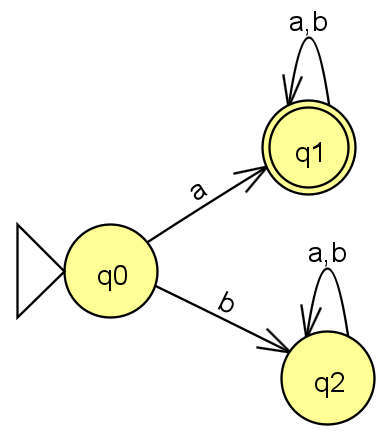
\includegraphics[width=0.2\textwidth]{../../../images/DFAs/ex1_q1.png}



% \vspace{3cm}
% \begin{flushleft}
% أرجو لكم وقتًا ممتعًا.

% الأستاذ محمود اغبارية.
% \end{flushleft}


% \end{document}


\ifwithsols
\title{حل أسئلة مراجعة قبل البرمجة الموجهة للكائنات (OOP)}
\else
\title{أسئلة مراجعة قبل البرمجة الموجهة للكائنات (OOP)}
\fi

\begin{document}

\maketitle
\thispagestyle{fancy}

\begin{enumerate}[itemsep=3em]

% Question 1: 2013_899222_3 (was Q3)
\item
معطاة مصفوفة \textenglish{arr} تحوي أعدادًا صحيحة.
اكتب قطعة برنامج تعدّ وتعرض كمُخرَج عدد الحدود في المصفوفة، التي القيمة المخزونة فيها (في الحدود) هي عدد مكوّن من رقمين.

\ifwithsols
\begin{boxSolution}
\begin{english}
\begin{minted}{csharp}
int count = 0;
for (int i = 0; i < arr.Length; i++)
{
    // Take absolute value in case numbers are negative
    int num = Math.Abs(arr[i]);
    if (num >= 10 && num <= 99)
        count++;
}
Console.WriteLine(count);
\end{minted}
\end{english}
\end{boxSolution}
\clearpage
\fi


% Question 2: 2003_899205_2 (was Q1)
\item
مصفوفة "تماثلية الجمع" هي مصفوفة تحقق الشرط التالي:
لكل أزواج الحدود - الحد الأول في المكان الـ $i$ من بداية المصفوفة والحد الآخر في المكان الـ $i$ من نهاية المصفوفة - يوجد نفس المجموع. أي، مجموع الحد الأول في المصفوفة والحد الأخير في المصفوفة يساوي مجموع الحد الثاني في المصفوفة والحد قبل الأخير في المصفوفة، وهكذا.

اكتب دالة ترجع قيمة بوليانية (\textenglish{bool}) تتلقى مصفوفة أحادية الأبعاد تحوي أعدادًا صحيحة بكبر $N$. \\
افترض أن $N$ هو عدد زوجي وأكبر من $0$. تقوم الدالة بفحص ما إذا كانت المصفوفة هي مصفوفة "تماثلية الجمع".

\textbf{مثال:} في المصفوفة التالية:
$$ [7, 3, 5, 4, 6, 2] $$
مجموع كل زوج حدود حسب الشرط هو 9. بالنسبة للمصفوفة، ترجع الدالة القيمة \textenglish{true}.

\ifwithsols
\begin{boxSolution}
\begin{english}
\begin{minted}{csharp}
public static bool IsSymmetricSum(int[] arr)
{
    int expectedSum = arr[0] + arr[arr.Length - 1];

    for (int i = 1; i < arr.Length / 2; i++)
    {
        if (arr[i] + arr[arr.Length - 1 - i] != expectedSum)
            return false;
    }

    return true;
}
\end{minted}
\end{english}
\end{boxSolution}
\fi


\clearpage
% Question 3: 2011_899222_10 (was Q2) modified
\item
ظهور سالب في المصفوفة هو تسلسل حدود قيمها سالبة. طول الظهور السالب هو عدد الحدود التي في الظهور السالب. يمكن أن يكون 1 أو أكثر. يمكن أن تشمل المصفوفة أكثر من ظهور سالب واحد.

اكتب عملية تتلقى مصفوفة تحوي أعدادًا صحيحة.
تُعيد العملية \textbf{فهرس (مؤشر) بداية أطول ظهور سالب} في المصفوفة. \\
إذا كان هناك أكثر من ظهور سالب بنفس الطول الأقصى، تُعيد فهرس بداية الظهور الأوّل من بينها. \\
إذا لم يكن هناك ظهور سالب في المصفوفة، تُعيد العملية $-1$.

\textbf{مثال:} بالنسبة للمصفوفة \textenglish{arr1} بكبر 10:
$$ [2, 5, -2, 7, 12, -3, -6, -17, -19, 2] $$
تُعيد العملية 5 (لأن أطول ظهور سالب يبدأ في الفهرس 5 وهو التسلسل $-3, -6, -17, -19$).

بالنسبة للمصفوفة \textenglish{arr2} بكبر 10:
$$ [12, 6, 7, -8, -11, -4, 7, 25, 9, 1] $$
تُعيد العملية 3 (لأن أطول ظهور سالب يبدأ في الفهرس 3 وهو التسلسل $-8, -11, -4$).
\textbf{ملاحظة:} لا حاجة لفحص سلامة المُدخلات.

\ifwithsols
\begin{boxSolution}
\begin{english}
\begin{minted}{csharp}
public static int LongestNegativeSequenceIndex(int[] arr)
{
    int maxLen = 0;
    int maxIndex = -1;
    int currentLen = 0;
    int currentIndex = -1;

    for (int i = 0; i < arr.Length; i++)
    {
        if (arr[i] < 0)
        {
            if (currentLen == 0)
                currentIndex = i;
            currentLen++;
        }
        else
        {
            if (currentLen > maxLen)
                maxLen = currentLen;
                maxIndex = currentIndex;
            currentLen = 0;
        }
    }

    // Final check in case the array ended with a negative sequence
    if (currentLen > maxLen)
        maxIndex = currentIndex;

    return maxIndex;
}
\end{minted}
\end{english}
\end{boxSolution}
\fi
\clearpage

% Question 4: Derived from classes accumulator (classes1_2026_899371_4)
\item
معطاة مصفوفتان متوازيتان بنفس الكبر:
المصفوفة الأولى \textenglish{productIds} تحوي أرقام منتجات (أعداد صحيحة بين 0 و 9). \\
المصفوفة الثانية \textenglish{quantities} تحوي كميات هذه المنتجات المطلوبة.

اكتب عملية تتلقى المصفوفتين \textenglish{productIds} و \textenglish{quantities}. \\
تُعيد العملية مصفوفة جديدة، بحيث يُحفظ في كل مكان (فهرس) $i$ في المصفوفة الجديدة مجموع الكميات المطلوبة للمنتج الذي رقمه $i$.

\textbf{مثال:}
المصفوفة \textenglish{productIds}: $[5, 3, 5, 8, 3, 5]$ \\
المصفوفة \textenglish{quantities}: $[10, 4, 3, 7, 2, 1]$ \\
في المصفوفة التي ستُعيدها العملية: \\
في المكان 5 ستكون القيمة 14 (لأن $10 + 3 + 1 = 14$). \\
في المكان 3 ستكون القيمة 6 (لأن $4 + 2 = 6$). \\
في المكان 8 ستكون القيمة 7. \\
في باقي الأماكن ستكون القيمة 0.

\ifwithsols
\begin{boxSolution}
\begin{english}
\begin{minted}{csharp}
public static int[] SumQuantities(int[] productIds, int[] quantities)
{
    int[] sums = new int[10];
    for (int i = 0; i < productIds.Length; i++)
    {
        sums[productIds[i]] += quantities[i];
    }
    return sums;
}
\end{minted}
\end{english}
\end{boxSolution}
\clearpage
\fi

% Question 5: Derived from classes unique elements (classes2_2026_899371_5)
\item
اكتب عملية تتلقى مصفوفة نصوص (\textenglish{string}) تحوي أسماءً. \\
تقوم العملية بطباعة جميع الأسماء "الفريدة" في المصفوفة، أي الأسماء التي تظهر مرّة واحدة فقط ولا تتكرر في أي مكان آخر في المصفوفة (يمكن طباعة الأسماء بأي ترتيب).

\textbf{مثال:}
بالنسبة للمصفوفة \textenglish{names}:
$$ [\text{"Amir"}, \text{"Sami"}, \text{"Amir"}, \text{"Rami"}, \text{"Huda"}, \text{"Sami"}] $$
تطبع العملية الاسمين: \\
\textenglish{Rami} \\
\textenglish{Huda} \\
لأنهما الاسمان الوحيدان اللذان يظهران مرة واحدة فقط في المصفوفة.

\ifwithsols
\begin{boxSolution}
\begin{english}
\begin{minted}{csharp}
public static void PrintUniqueNames(string[] names)
{
    for (int i = 0; i < names.Length; i++)
    {
        bool isUnique = true;
        for (int j = 0; j < names.Length; j++)
        {
            if (i != j && names[i] == names[j])
                isUnique = false;
        }

        if (isUnique)
            Console.WriteLine(names[i]);
    }
}
\end{minted}
\end{english}
\end{boxSolution}
\fi

\clearpage
% Question 6: Unique last 2 digits
\item
اكتب عملية تتلقى مصفوفة أعداد صحيحة (\textenglish{int}). \\
تقوم العملية بطباعة جميع الأعداد في المصفوفة التي تملك منزلتين يمنيين (آحاد وعشرات) "فريدة"، أي لا يوجد أي عدد آخر في المصفوفة يملك نفس منزلة الآحاد والعشرات.

\textbf{مثال:}
بالنسبة للمصفوفة:
$ [145, 203, 345, 908, 12] $
تطبع العملية الأعداد: \\
$203$ (لأن $03$ لا يتكرر في أعداد أخرى) \\
$908$ (لأن $08$ لا يتكرر) \\
$12$ (لأن $12$ لا يتكرر) \\
ملاحظة: العددين 145 و 345 يملكان نفس الآحاد والعشرات (45)، لذلك لا تتم طباعتهما.

\ifwithsols
\begin{boxSolution}
\begin{english}
\begin{minted}{csharp}
public static void PrintUniqueLastTwoDigits(int[] arr)
{
    for (int i = 0; i < arr.Length; i++)
    {
        bool isUnique = true;
        for (int j = 0; j < arr.Length; j++)
        {
            if (i != j && Math.Abs(arr[i]) % 100 == Math.Abs(arr[j]) % 100)
                isUnique = false;
        }

        if (isUnique)
            Console.WriteLine(arr[i]);
    }
}
\end{minted}
\end{english}
\end{boxSolution}
\fi

\end{enumerate}

\vspace{1cm}
\begin{flushleft}
أرجو لكم وقتًا ممتعًا.

الأستاذ محمود اغبارية.
\end{flushleft}

\end{document}
